\documentclass[10pt]{article}

% ============================================================================
% CSC manuscript — NEUTRAL build (self-contained, compiles with base LaTeX).
% Story: identifiability/abstention boundary -> Route A Z-only frozen NEGATIVE
%        -> Route B3 paired minimal-label frozen POSITIVE (synthetic).
% Two-build convention (mirrors tos_cmi/paper): this main.tex is venue-neutral;
% a venue stylefile build (venue_main.tex + <venue>.sty) drops in once the
% venue is fixed -- see README.md. Do NOT hardcode a venue here.
% ============================================================================

\usepackage[margin=1in]{geometry}
\usepackage{times}
\usepackage{amsmath,amssymb,amsfonts}
\usepackage{graphicx}
\usepackage{booktabs}
\usepackage{tabularx}
\usepackage{xcolor}
\usepackage{natbib}
\usepackage{hyperref}
\usepackage{caption}
\usepackage{subcaption}
\usepackage{amsthm}

\graphicspath{{figures/}}

\newtheorem{proposition}{Proposition}
\newtheorem{assumption}{Assumption}

% --- draft-mode claim tags: traceability to claim_evidence_table.md, HIDDEN in PDF ---
\newif\ifshowclaimtags
\showclaimtagsfalse
\newcommand{\claimtag}[1]{\ifshowclaimtags\textcolor{blue}{[#1]}\fi}

% --- draft-mode TODO notes: VISIBLE in draft, flip to hide for a clean build ---
\newif\ifshowtodo
\showtodotrue
\newcommand{\todo}[1]{\ifshowtodo\textcolor{red}{\textbf{[TODO: #1]}}\fi}

% state-name shorthand (exact certifier states)
\newcommand{\stcov}{\textsc{Covariate\_Compatible}}
\newcommand{\stsus}{\textsc{Concept\_Suspect}}
\newcommand{\stunid}{\textsc{Unidentifiable}}
\newcommand{\stconf}{\textsc{Concept\_Confirmed}}
\newcommand{\stnoev}{\textsc{No\_Concept\_Evidence}}
\newcommand{\stneed}{\textsc{Need\_More\_Labels}}
\newcommand{\stinv}{\textsc{Invalid\_Pair\_Structure}}

\title{When Can EEG Concept Shift Be Certified?\\
From \texorpdfstring{$Z$}{Z}-only Abstention to Paired Minimal-Label Certificates}
\author{Anonymous}
\date{}

\begin{document}
\maketitle

\begin{abstract}
We study \emph{when} a concept shift --- a change in the class posterior $P(Y\mid Z)$ of a learned
representation --- can be \emph{certified} at deployment time, and when a method must instead abstain. We
treat this as an identifiability problem rather than a detection benchmark, using clinical EEG (scarce
labels, plentiful unlabeled target recordings) as the motivating high-stakes setting. We first prove that
concept shift is not identifiable from the unlabeled target marginal $Z$ alone: for any observed marginal
there exist joint laws with identical $Z$ but different posteriors (Prop.~\ref{prop:impossible}), so
abstention is a necessary output, not a design weakness. We then contrast two operating regimes under a
single, shared discipline of \emph{freeze-before-confirmatory} evaluation. \textbf{Route A} is a
source-anchored, $Z$-only certificate: in development sweeps it exhibited an apparent identifiable core,
but a frozen confirmatory test on unseen synthetic clusters \emph{failed both} the false-certification and
the power endpoints --- an audited negative result that surfaces, rather than hides, an
informed-selection/generalization gap. \textbf{Route B3} adds a small, targeted amount of information --- of the kind
Prop.~\ref{prop:impossible} shows is required: a \emph{paired within-subject} target-internal reference (each subject's own
alternative condition) plus a few labels. A pre-registered, frozen, unseen-cluster synthetic confirmatory
of the Route-B3 certificate \emph{passed} all criteria within its declared operating envelope: false
confirmation stayed within the pre-declared pointwise control gates and primary concept-shift power was
$1.00$. The contribution is a formal and empirical \emph{boundary} for EEG concept-shift certification ---
a $Z$-only impossibility with an audited negative confirmatory, and a minimal-information (paired,
few-label) positive confirmatory --- together with the freeze-before-confirmatory audit protocol that
produced both verdicts. All results are on synthetic data; real-EEG validation is future work.
\end{abstract}

\section{Introduction}
\label{sec:intro}

\todo{Full prose pass. Skeleton below fixes the claims, scope, and contributions; expand each bullet into
1--2 paragraphs and add citations (see references.bib stubs).}

\paragraph{Problem.}
When an EEG model trained on a source population is deployed on a new target (new subjects, sites, or
conditions), the practical question is not only ``did the input distribution move'' but ``did the
\emph{decision rule} $P(Y\mid Z)$ move'' --- a \emph{concept shift}. A tempting goal is a universal,
label-free detector that reads concept shift off the unlabeled target embeddings $Z$.
\claimtag{C-motivation}
We show this goal is not attainable in general, reframe the object as a \emph{certificate with explicit
abstention}, and ask the sharper question: \emph{what is the minimal information that turns abstention into
a confirmable certificate, and does that certificate survive a frozen confirmatory test?}

\paragraph{Two regimes, one discipline.}
We compare two certificates under an identical audit protocol (development $\rightarrow$ freeze
tag$+$manifest$+$fail-closed runner $\rightarrow$ single unseen confirmatory):
\begin{itemize}
  \item \textbf{Route A} --- a source-anchored, $Z$-only certificate. Its frozen confirmatory is a
        \emph{negative} result (Sec.~\ref{sec:routeA}): the development-observed core did not generalize.
  \item \textbf{Route B3} --- a paired within-subject, minimal-label certificate that supplies exactly the
        extra information Prop.~\ref{prop:impossible} shows is missing. Its frozen confirmatory is a
        \emph{positive} result within a pre-registered synthetic envelope (Sec.~\ref{sec:routeB3conf}).
\end{itemize}

\paragraph{Contributions.}
\begin{enumerate}
  \item \textbf{Impossibility + abstention (Sec.~\ref{sec:theory}).} A $Z$-only certificate cannot decide
        concept shift for \emph{any} observed marginal (Prop.~\ref{prop:impossible}); the honest output is
        three-state with an \stunid{} (abstain) branch.
        \claimtag{C-impossible}
  \item \textbf{An audited negative (Sec.~\ref{sec:routeA}).} A frozen confirmatory falsifies a plausible
        $Z$-only development core --- forbidden (false-cert) rate above $\alpha$ \emph{and} power below the
        deployment bar on unseen clusters.
        \claimtag{C-routeA-neg}
  \item \textbf{A minimal-information positive (Secs.~\ref{sec:routeB3method}--\ref{sec:routeB3conf}).}
        A paired within-subject target-internal reference plus a few labels yields a certificate whose
        frozen unseen-cluster synthetic confirmatory passes all pre-registered criteria within its declared
        envelope (primary power $1.00$; false confirmation within the pointwise control gates).
        \claimtag{C-routeB3-pos}
  \item \textbf{The audit protocol as a contribution (Sec.~\ref{sec:routeB3conf}, appendix).}
        Freeze-before-confirmatory with non-selection rules, conservative denominators, fail-closed
        provenance, and an independent red-team re-aggregation --- the same machinery yields the negative
        \emph{and} the positive verdict, which is why both are credible.
        \claimtag{C-protocol}
\end{enumerate}

\paragraph{Scope (stated up front).}
All results are \textbf{synthetic}. Route B3's positive claim holds within a \emph{development-informed,
frozen-before-confirmatory} operating envelope (Sec.~\ref{sec:routeB3conf}); it is not a claim that concept
shift is solved in general, nor a real-EEG result. Real EEG (e.g.\ Parkinson's ON/OFF paired recordings)
is future work requiring its own freeze and authorization (Sec.~\ref{sec:discussion}).

\section{Theory: non-identifiability and the necessity of abstention}
\label{sec:theory}

\todo{Tighten proof prose; confirm notation matches Sec.~4--5; add related-work pointers for
partial identification. Content below is locked to csc/THEORY.md.}

\paragraph{Setup.}
Let $Z$ be a fixed representation of an EEG epoch and $Y$ the label. The source law is $P_S(Z,Y)$; a target
provides samples of $Q_Z$ (the unlabeled target marginal), and in the minimal-label regimes of
Sec.~\ref{sec:routeB3method} a small number of target labels. A \emph{concept shift} is a change in the
posterior, $Q(Y\mid Z)\neq P_S(Y\mid Z)$.

\subsection{A $Z$-only certificate cannot identify concept shift}

\begin{proposition}[No $Z$-only concept identification]
\label{prop:impossible}
Fix any target marginal $Q_Z$. There exist two joint target laws $Q_0,Q_1$ with
$Q_0(Z)=Q_1(Z)=Q_Z$ but $Q_0(Y\mid Z)=P_S(Y\mid Z)$ and $Q_1(Y\mid Z)\neq P_S(Y\mid Z)$. Any certificate
that is a function of the unlabeled target (a function of $Q_Z$) returns the same value on $Q_0$ and $Q_1$.
Hence no $Z$-only certificate can decide ``$P(Y\mid Z)$ unchanged'' vs.\ ``concept shift'' --- for
\emph{any} observed marginal, not only when $Q_Z=P_S(Z)$.
\end{proposition}

\begin{proof}
Pick any $Q_Z$ with full support on the source $Z$-support and set $Q_0(Y\mid Z)=P_S(Y\mid Z)$. For $Q_1$,
perturb the posterior on a positive-measure set (e.g.\ swap two classes' posteriors on a region) while
keeping the same $Q_Z$; both are valid joints with marginal $Q_Z$. A $Z$-only $f$ sees $Q_Z$ in both cases,
so $f(Q_0)=f(Q_1)$ and is wrong on at least one. \qed
\end{proof}

\paragraph{Consequence.}
``The target marginal landed in a concept direction'' is, on its own, \emph{not} identification of concept
shift; it is only \emph{evidence} under an extra, explicit assumption that ties what the source showed to
what the target is doing.

\begin{assumption}[atlas transportability + signature separability]
\label{ass:T}
(i) The target shift is generated by the same mechanism family the source spans --- its marginal signature
lies in the span of the source covariate/concept/label signatures (no novel mechanism); and (ii) those
signature subspaces are separable (a covariate-only move and a boundary-moving concept change leave
distinguishable marginal traces).
\end{assumption}

Under Assumption~\ref{ass:T} a marginal certificate is a \emph{conditional, abstention-equipped partial
identification} statement, never distribution-free identification --- and it must abstain whenever the
target leaves the atlas (Prop.~\ref{prop:impossible}'s ``novel direction'' branch).

\subsection{The shift taxonomy and the three-state output}

\begin{table}[t]
\centering
\caption{Shift taxonomy. Only a $Z$-visible \emph{and} source-anchored trace admits a (conditional)
certificate; pure conditional and label shift are $Z$-only-unidentifiable and must abstain.}
\label{tab:taxonomy}
\begin{tabular}{@{}llll@{}}
\toprule
shift & $P(Z)$ & $P(Y\mid Z)$ & marginal-only certificate \\
\midrule
covariate                 & changes (nuisance) & invariant & \stcov{} \\
boundary-coupled concept  & changes            & changes   & \stsus{} (under Assumption~\ref{ass:T}) \\
pure conditional concept  & invariant          & changes   & \stunid{} (Prop.~\ref{prop:impossible}) \\
label (target) shift      & changes            & changes   & \stunid{} \\
\bottomrule
\end{tabular}
\end{table}

Table~\ref{tab:taxonomy} forces a \textbf{three-state} $Z$-only output --- \stcov{} / \stsus{} / \stunid{}
--- never a binary detector. \stcov{} is a \emph{compatibility} claim (source boundary stable in the moved
subspace), not an adaptation guarantee. The label-shift row is the sharpest trap: a change in $P(Y)$ with
$P(Z\mid Y)$ fixed moves the pooled mean along the class-mean subspace and mimics concept movement, so the
certifier carries an explicit label subspace and label gate and abstains there.

\begin{figure}[t]
\centering
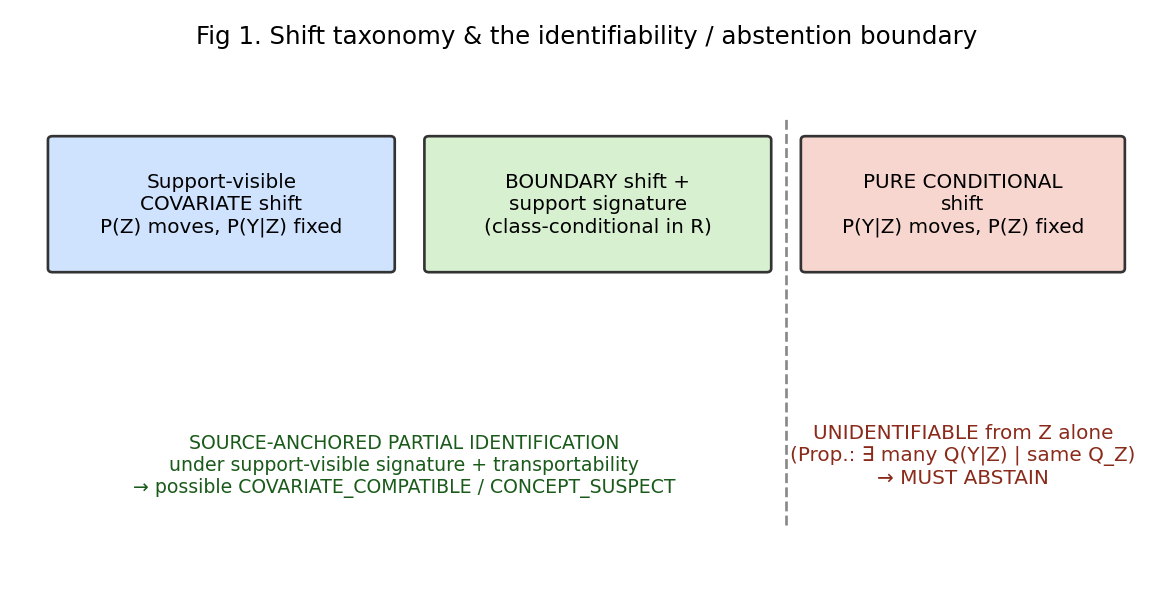
\includegraphics[width=0.86\linewidth]{fig1_taxonomy_boundary.png}
\caption{Shift taxonomy and the identifiability/abstention boundary: $Z$-visible, source-anchored traces
admit a conditional certificate; invisible/label-confounded/out-of-atlas shifts fall in the abstention
region (Prop.~\ref{prop:impossible}).}
\label{fig:taxonomy}
\end{figure}

\paragraph{What is proven vs.\ assumed (honesty).}
\emph{Proven} (Prop.~\ref{prop:impossible}): a $Z$-only certificate cannot identify concept shift for any
marginal. \emph{Assumed/open}: Assumption~\ref{ass:T} (transportability + separability) is untestable from
the target marginal alone; a marginal \stsus{} is therefore source-anchored suspicion under an explicit
assumption. This is precisely the gap that motivates supplying a small amount of \emph{additional information} in
Sec.~\ref{sec:routeB3method}.

\section{Route A: a source-anchored $Z$-only certificate, and its frozen negative}
\label{sec:routeA}

\todo{Expand method subsection from csc/THEORY.md \S3--\S4 (statistic, parametric-bootstrap null, support
gate, atlas/direction-linked evidence). Keep the confirmatory numbers exactly as below (verified against
csc/results/confirmatory.json).}

\subsection{Certificate design (summary)}
Route A instantiates the three-state output of Sec.~\ref{sec:theory} as a \emph{source-anchored} certificate:
a source-side concept statistic with a parametric-bootstrap null under the fitted no-shift model $h_0$; a
\emph{support gate} (bipartite connectivity + minimum cell counts + design conditioning) that abstains on
disconnected/rank-deficient designs; a low-moment \emph{atlas} of covariate/concept/label subspaces with
direction-linked concept evidence; and a label subspace/gate for the label-shift trap
(Table~\ref{tab:taxonomy}). The analysis unit is the subject (cluster-valid inference throughout). Under
Assumption~\ref{ass:T} it emits \stcov{}/\stsus{}, and abstains (\stunid{}) otherwise. \claimtag{C-routeA-design}

\subsection{Development sweep suggested an identifiable core}
A pre-registered difficulty-envelope sweep (star design over effect size, subjects, epochs, correlation,
imbalance, leakage, mechanism family) located an apparent favourable operating point $P_{\text{baseline}}$
(concept effect $14$, $22$ subjects/domain, $30$ target subjects, balanced priors, correlation $0.2$,
covariate leakage $10$, $3$ concept domains, $22$ epochs). Crucially, the development map \emph{itself}
flagged that $12$ clusters/cell give only a Clopper--Pearson upper bound $\approx 0.221$ on the forbidden
rate --- a boundary locator, \textbf{not} error control. \claimtag{C-routeA-dev}

\subsection{The frozen confirmatory falsifies the core}
We froze the method (tag, manifest hash, fail-closed runner) and ran a single confirmatory on \emph{unseen}
clusters (base seed $900000$; source seeds $900000\text{--}900065 \rightarrow$ target seeds
$1800000\text{--}1800065$, disjoint). The pre-registered headline is a conjunction of a false-certification
gate and a power gate. Both failed (Table~\ref{tab:routeA}). \claimtag{C-routeA-neg}

\begin{table}[t]
\centering
\caption{Route A, same operating point $P_{\text{baseline}}$, evaluated two ways. The frozen confirmatory
($\geq 59$ valid clusters; $0$-failure CP-UB $\leq 0.05$; power bar $0.50$ with a
$\max(\text{conditional},\text{unconditional})$ guard) refutes the development core:
\texttt{headline\_core\_pass=false}.}
\label{tab:routeA}
\begin{tabular}{@{}lll@{}}
\toprule
 & development (P1.5 map, dev seeds) & confirmatory (frozen, unseen seed $900000$) \\
\midrule
clusters                 & $12$/cell                 & $G=66$, $N_{\text{valid}}=65$ \\
visible-concept power     & $0.83$ (CP-LB $0.56$)     & $\mathbf{0.43}$ ($28/65$; CP-LB $\mathbf{0.326}$) \\
forbidden (false-cert)    & $0/12$                    & $\mathbf{1/65}$, CP-UB $\mathbf{0.0709} > \alpha{=}0.05$ \\
headline                  & apparent favourable core  & \textbf{FAIL both endpoints} \\
\bottomrule
\end{tabular}
\end{table}

\begin{figure}[t]
\centering
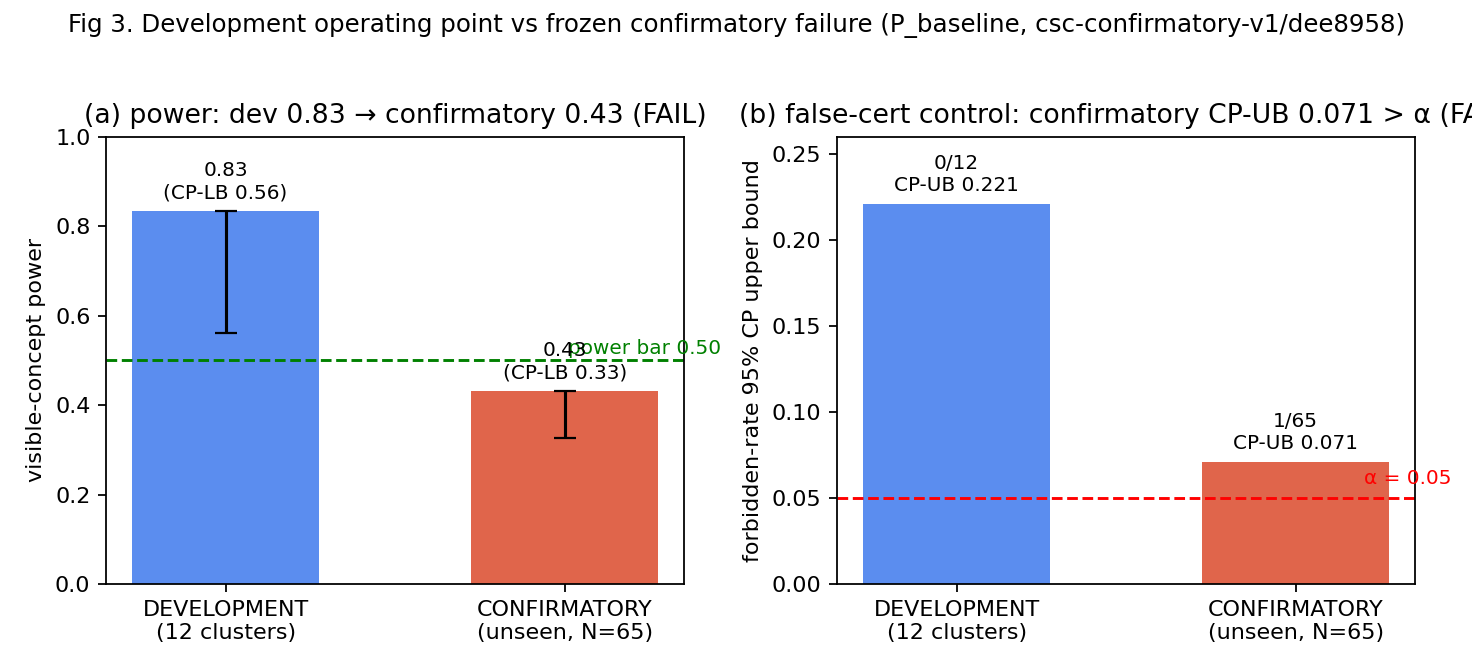
\includegraphics[width=0.9\linewidth]{fig3_dev_vs_confirmatory.png}
\caption{Route A development operating map vs.\ frozen confirmatory: the development-favourable region does
not reproduce on unseen clusters (power drops, forbidden rate exceeds $\alpha$). The gap is an
informed-selection/generalization effect \emph{surfaced} by the freeze$\rightarrow$unseen protocol.}
\label{fig:devconf}
\end{figure}

\paragraph{Reading.}
The negative is not a bug: it is the freeze-before-confirmatory protocol doing its job. Per protocol the
result was committed and \emph{not} rerun; no threshold, seed, manifest, or tag was changed. Route A
establishes that a plausible, heavily engineered $Z$-only development core can fail both endpoints on unseen
data --- consistent with Prop.~\ref{prop:impossible}: without extra information tying source evidence to the
target posterior, marginal concept evidence is fragile. This motivates Route B3. \claimtag{C-routeA-read}

\section{Route B3: a paired within-subject, minimal-label certificate}
\label{sec:routeB3method}

\todo{Expand each component into method prose + a small algorithm box; add the pipeline figure caption
cross-ref. All parameter values below are the frozen method lock (calibration\_version
\texttt{p24d\_cross\_budget\_alpha\_spending\_studentized\_fixed\_margin}).}

\paragraph{The missing information.}
Prop.~\ref{prop:impossible} says the target marginal is insufficient. Route B3 supplies the minimal extra
information that breaks the tie: (i) a \emph{paired within-subject reference} --- each subject contributes
two conditions (e.g.\ ON/OFF), so the subject is their \emph{own} control and the subject random effect
cancels; and (ii) a \emph{few labels} on eligible paired subjects. Critically, the reference is
\emph{target-internal}: no source posterior is used, so Route B3 sidesteps the source-reference
contamination and covariate-extrapolation failure modes that make a source-anchored certificate fragile. \claimtag{C-b3-idea}

\paragraph{Conditional-change test.}
For a subject with conditions indexed by a centered code $c\in\{-\tfrac12,+\tfrac12\}$, we compare
\[
h_0:\ [\,Z,\ c\,] \qquad\text{vs.}\qquad h_1:\ [\,Z,\ c,\ c\times Z_{\mathrm{pc}}\,]
\]
where $Z_{\mathrm{pc}}$ is a low-rank (rank $3$) principal-component basis and the $c\times Z_{\mathrm{pc}}$
interaction is the condition-dependent boundary change. The statistic is a subject-condition-vote
difference of negative log-likelihoods, $T=\mathrm{vote}(\mathrm{NLL}_{h_0})-\mathrm{vote}(\mathrm{NLL}_{h_1})$,
cross-fitted over $3$ folds. Centered ($\pm\tfrac12$) coding is essential: $0/1$ coding makes the
interaction asymmetric and induces a type-I failure. \claimtag{C-b3-test}

\paragraph{Calibrated inference (the method lock).}
The frozen certifier (\texttt{pc\_centered\_calibrated}) combines:
\begin{itemize}
  \item \textbf{Pair-integrity + eligibility guards}: pair integrity $\geq 0.95$; an eligible complete pair
        needs $\geq 8$ epochs per condition; per-condition class coverage required, else \stinv{}/\stneed{}.
  \item \textbf{Condition-matched fixed-margin $h_0$ bootstrap}: within-condition label swaps that preserve
        the per-condition class margins (Metropolis, acceptance $\propto p_0$); $n_{\text{boot}}=200$;
        invalid replicates are \emph{counted}, not dropped.
  \item \textbf{Studentized subject-consistency gate}: $Z=\overline{\Delta}_s/\mathrm{se}(\Delta_s)$ over
        per-subject deltas, requiring the lower confidence bound on $\overline{\Delta}_s$ to exceed $0$.
  \item \textbf{Cross-budget $\alpha$-spending}: family $\alpha=0.05$ split over the two positive-decision
        budgets $m\in\{20,30\}$, giving $\alpha_{\text{budget}}=0.025$ on the $p$-gates and a $0.975$ LCB.
\end{itemize}
A positive decision at budget $m$ requires the fixed-margin mean-$T$ $p\leq\alpha_{\text{budget}}$
\emph{and} the studentized $p\leq\alpha_{\text{budget}}$ \emph{and} $\mathrm{LCB}_{0.975}(\Delta_s)>0$.

\paragraph{Output states.}
Route B3 emits \stconf{} / \stnoev{} / \stneed{} / \stinv{} / \stunid{} --- there is no \stcov{} state
(covariate compatibility is not a Route-B3 claim). The design fails closed: unsound pairing, too few
epochs, or too few eligible labelled subjects yield abstention, never a confirmation. \claimtag{C-b3-states}

\begin{figure}[t]
\centering
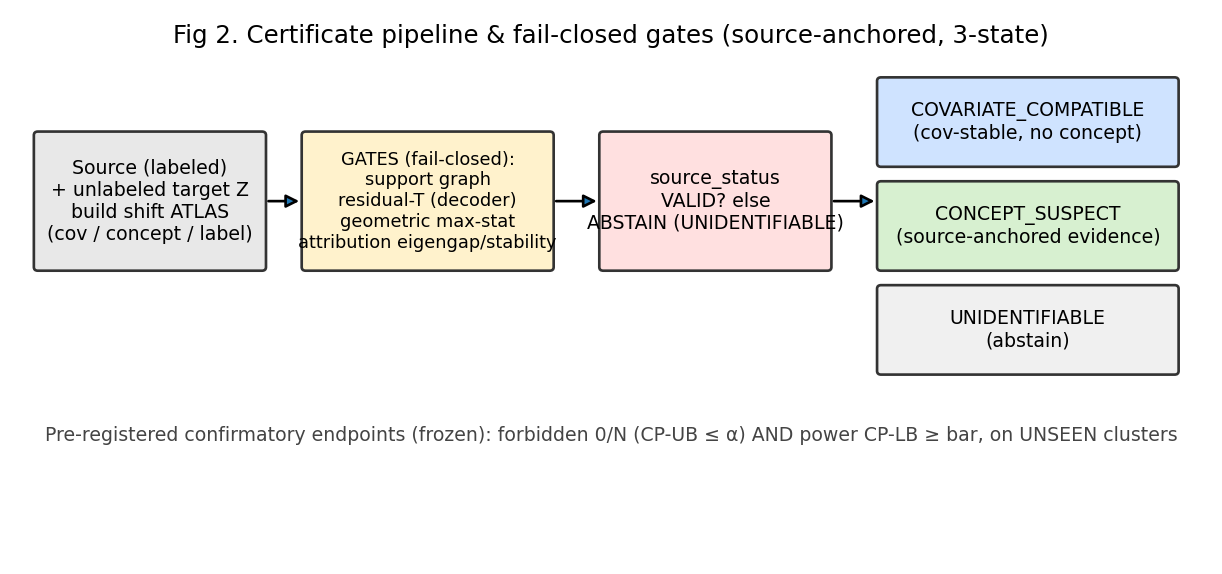
\includegraphics[width=0.92\linewidth]{fig2_pipeline_gates.png}
\caption{Certificate pipeline and fail-closed gates. \todo{Regenerate a B3-specific pipeline figure:
paired within-subject ON/OFF $\rightarrow$ pair-integrity/eligibility guards $\rightarrow$ centered
conditional-change test $\rightarrow$ fixed-margin null $+$ studentized gate $+$ cross-budget
$\alpha$-spending $\rightarrow$ \{\stconf, \stnoev, \stneed, \stinv, \stunid\}. Current figure is the
Route-A pipeline placeholder.}}
\label{fig:pipeline}
\end{figure}

\section{Route B3 frozen confirmatory: a minimal-information positive}
\label{sec:routeB3conf}

\todo{Add prose framing around the tables; move full per-cell dumps + C6 red-team detail to the appendix if
space is tight. All numbers below are verified against csc/results/b3\_confirmatory\_result.json
(tag csc-b3-confirmatory-v1, commit 0595f64, manifest a96dc0de).}

\subsection{Pre-registration and provenance}
The Route-B3 method was frozen (method lock, machine-readable manifest, canonical hash, deterministic seed
schedule, fail-closed runner) and a \emph{single} confirmatory was run on unseen synthetic clusters. Base
seed $3000000$; $5376$ clusters ($112$ cells $\times$ $48$ replicates); seed range
$[3000000,14100047]$, disjoint from the Route-A source/target seeds, the development seeds, and the
smoke/test range. Provenance was verified (frozen tree clean, running code hash $=$ manifest, HEAD $=$ tag
commit) and the artifact was independently re-aggregated by a red-team (Sec.~\ref{sec:b3-c6}). \claimtag{C-b3-prov}

\subsection{The claim and its envelope}
\textbf{Primary claim (scoped).} On paired within-subject targets with sound pairing (integrity $\geq 0.95$,
$\geq 8$ epochs/condition) and $\geq 20$ eligible labelled paired subjects, the certifier confirms genuine
class-conditional/boundary concept shift (\texttt{paired\_concept}, \texttt{paired\_concept\_plus\_cov})
while controlling false confirmation at $\alpha$ --- within the pre-registered envelope: scenarios
\{baseline, high\_nuisance, high\_subject\_tau, imbalanced\}, budgets $m\in\{20,30\}$. \emph{Controls} are
evaluated over \emph{all six} stress scenarios (including \texttt{label\_noise} and \texttt{few\_epochs}).
Heavy label noise and very-short-record regimes are \textbf{pre-registered out} of the primary
\emph{power} claim (declared, not discovered afterward). \claimtag{C-b3-envelope}

\subsection{Confirmatory criteria (all pass)}
The verdict is a conjunction $C_1\wedge\dots\wedge C_6$ (Table~\ref{tab:b3criteria}).

\begin{table}[t]
\centering
\caption{Route B3 frozen confirmatory, unseen clusters: $C_1$--$C_6$ all pass.}
\label{tab:b3criteria}
\begin{tabularx}{\linewidth}{@{}llX@{}}
\toprule
criterion & result & headline number \\
\midrule
$C_1$ guards (no false confirm) & PASS & \texttt{missing\_pair} $0/576$, \texttt{unequal\_epochs} $0/576$ \\
$C_2$ control type-I (kind$\times$budget, $n{=}288$, CP-up $\leq .05$) & PASS & worst \texttt{clean}$|$m30 $=3/288$, CP-up $\mathbf{0.0267}$ \\
$C_3$ no hot cell / no kind-leak & PASS & max control cell $2/48$; $0$ cells $\geq 6$; $0$ cells $\geq 3$ \\
$C_4$ primary power (kind$\times$budget, $n{=}192$, CP-lo $\geq .60$) & PASS & all four $=\mathbf{1.000}$, CP-lo $\mathbf{0.9845}$ \\
$C_5$ no silent failure & PASS & sampler $0$, boot-invalid $0$, $0$ out-of-set states \\
$C_6$ red-team reproduces without correction & PASS & independent re-aggregation matches (Sec.~\ref{sec:b3-c6}) \\
\bottomrule
\end{tabularx}
\end{table}

\paragraph{$C_2$ --- control false confirmation (all 14 cells, $n=288$ each, pooled over 6 scenarios).}
Denominators are conservative (\stneed{}/\stinv{} retained). Stratified by budget, not pooled across
budgets. Every CP-upper $\leq 0.05$; total control confirmations $=6$.

\begin{table}[t]
\centering
\caption{$C_2$: control kind $\times$ budget, false-confirmation counts and one-sided $0.95$ CP-upper.}
\label{tab:b3c2}
\begin{tabular}{@{}lcccc@{}}
\toprule
control kind & m20 & CP-up & m30 & CP-up \\
\midrule
clean                          & $1/288$ & $0.0164$ & $\mathbf{3/288}$ & $\mathbf{0.0267}$ \\
paired\_covariate              & $0/288$ & $0.0103$ & $1/288$ & $0.0164$ \\
paired\_label                  & $0/288$ & $0.0103$ & $0/288$ & $0.0103$ \\
random\_label                  & $0/288$ & $0.0103$ & $0/288$ & $0.0103$ \\
paired\_covariate\_plus\_label & $1/288$ & $0.0164$ & $0/288$ & $0.0103$ \\
missing\_pair (guard)          & $0/288$ & $0.0103$ & $0/288$ & $0.0103$ \\
unequal\_epochs\_extreme (guard)& $0/288$ & $0.0103$ & $0/288$ & $0.0103$ \\
\bottomrule
\end{tabular}
\end{table}

\paragraph{$C_4$ --- primary power (all 4 gating cells, $n=192$ each, pooled over the 4 strong scenarios).}
Both concept kinds, both budgets: power $192/192=1.000$, CP-lower $0.9845$. Every per-scenario cell
($n=48$) is $1.00$, so the $\geq 0.50$ per-cell floor holds everywhere.

\subsection{Secondary, non-gating: the pure-conditional tail stays weak}
The invisible pure-conditional relabel (\texttt{paired\_pure\_conditional}) remains hard even with the full
machinery: power $42/288=0.146$ (m20) and $81/288=0.281$ (m30). This is \emph{reported, not gating}: Route
B3's primary success is paired class-conditional/boundary concept shift, \textbf{not} all pure conditional
shift. \claimtag{C-b3-secondary}

\subsection{Independent red-team re-aggregation ($C_6$)}
\label{sec:b3-c6}
A separate agent re-aggregated all $5376$ per-cluster records from scratch (its own Clopper--Pearson
implementation), verified the seed schedule, canonical manifest hash, code provenance, denominators, and
state accounting, and reproduced $C_1$--$C_5$ \emph{without correction} (CP agreement to machine precision,
$\max|\Delta|\approx 2.8\times10^{-17}$; no denominator inflation; controls confirmed evaluated over all $6$
scenarios; confirmed-count accounting $6+768+123=897$ reconciles). The same audit machinery produced the
Route-A negative (Sec.~\ref{sec:routeA}) and this positive, which is why both verdicts are credible. \claimtag{C-b3-c6}

\paragraph{Reading.}
Within its declared synthetic envelope, adding a paired within-subject target-internal reference plus a few
labels moves the certificate from \stunid{} to a \emph{confirmable} \stconf{} that survives a frozen,
unseen-cluster, independently red-teamed test. This is the minimal-information positive counterpart to the
Route-A negative --- not a general solution (Sec.~\ref{sec:discussion}). The two routes are contrasted on the
pre-registered endpoints in Fig.~\ref{fig:evidence}.

\begin{figure*}[t]
\centering
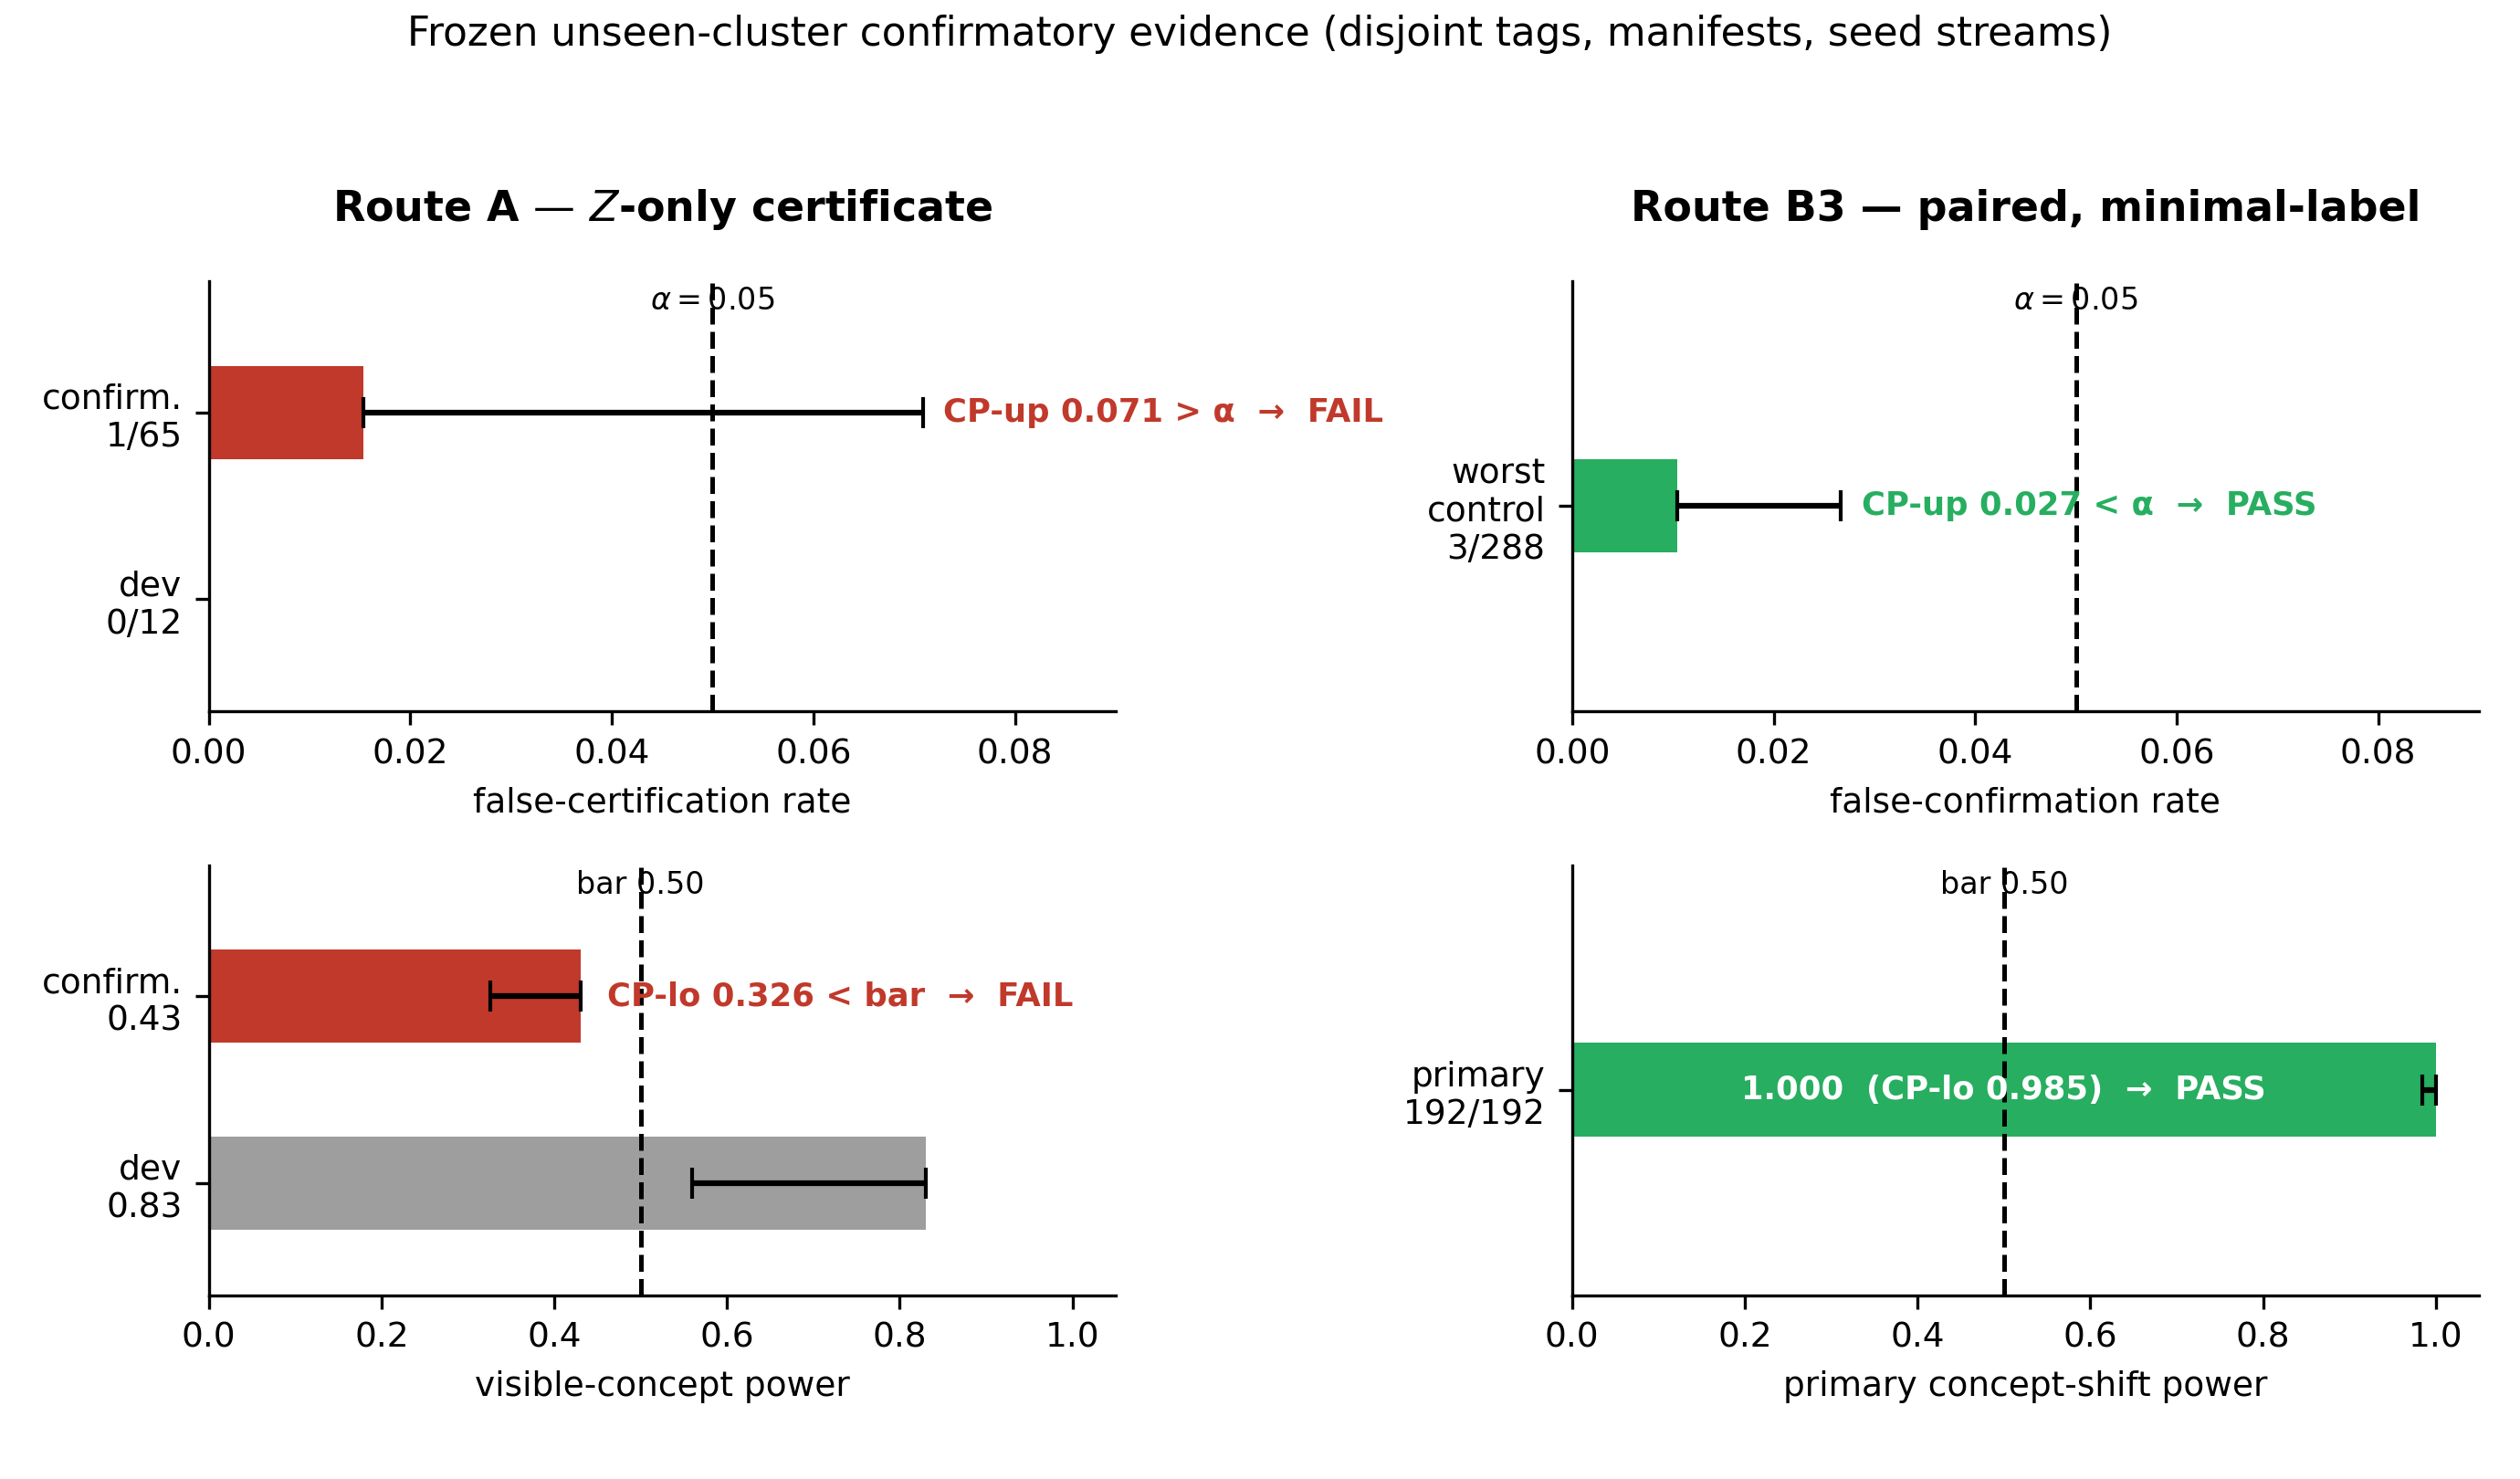
\includegraphics[width=0.95\linewidth]{fig3_routeA_negative_B3_positive.png}
\caption{Frozen confirmatory evidence: Route A (left, $Z$-only) vs.\ Route B3 (right, paired minimal-label),
on the two pre-registered endpoints --- \emph{top}: false-certification/confirmation rate against
$\alpha=0.05$; \emph{bottom}: concept-shift power against the $0.50$ bar. \textbf{Both columns are frozen
confirmatory results on unseen clusters, not development estimates}, and the two routes use \emph{disjoint}
tags, manifests, and seed streams (Route~A \texttt{csc-confirmatory-v1}, base seed $900000$; Route~B3
\texttt{csc-b3-confirmatory-v1}, base seed $3000000$). Route~A fails both endpoints (false-cert CP-upper
$0.071>\alpha$; power $0.43$, CP-lower $0.326<0.50$; \texttt{headline\_core\_pass=false}); Route~B3 passes
both (worst control CP-upper $0.027<\alpha$; primary power $1.000$, per-cell CP-lower $0.985$), with guards
$0/576$, no silent failures ($C_5$), and the $C_6$ red-team reproducing the verdict without correction. Error
bars are one-sided Clopper--Pearson bounds; grey bars show the Route~A \emph{development} point for contrast.}
\label{fig:evidence}
\end{figure*}

\section{Related work}
\label{sec:related}

\todo{Draft after abstract lock; add real citations to references.bib. Position against: (i) distribution
shift / domain generalization and the covariate-vs-concept distinction; (ii) label-shift estimation and why
it is the sharpest trap here; (iii) partial identification / bounds under untestable assumptions; (iv) EEG
domain generalization and cross-subject/cross-site transfer; (v) pre-registration / frozen-evaluation
discipline in ML.}

\paragraph{Distribution shift and the concept-shift subclass.}
\todo{Covariate vs concept shift; why label-free concept detection is the hard subcase.}
\cite{placeholder_dg}

\paragraph{Label shift.}
\todo{Estimation/correction; contrast with our abstention on the label-shift row (Table~\ref{tab:taxonomy}).}
\cite{placeholder_labelshift}

\paragraph{Partial identification.}
\todo{Bounds/certificates under untestable assumptions; our three-state output as a partial-identification
device.}
\cite{placeholder_partialid}

\paragraph{EEG domain generalization.}
\todo{Cross-subject/cross-site transfer; where paired within-subject designs (e.g.\ ON/OFF) fit.}
\cite{placeholder_eegdg}

\section{Discussion, boundary, and limitations}
\label{sec:discussion}

\paragraph{What the two routes jointly establish.}
Route~A and Route~B3 are not contradictory results; together they trace an \emph{information boundary} for
concept-shift certification. Route~A shows that an unlabeled target marginal --- even when mined by a strong,
source-anchored, fail-closed certificate --- does not carry enough information to certify a conditional shift,
and that a development-favourable operating core need not survive a frozen test. Route~B3 shows that adding a
small, targeted amount of target-side information (a paired within-subject reference plus a few labels) changes
the statistical problem from unidentifiable to confirmable, moving the certificate from \stunid{} to a
frozen-confirmed \stconf{}. The result is a ladder from abstention to confirmation, indexed by \emph{what is
observed}, rather than a single detector.

\paragraph{Why the negative matters.}
The Route~A negative is not a failed baseline to be discarded; it is load-bearing. It is the empirical
counterpart of Proposition~\ref{prop:impossible}: without extra information tying source evidence to the
target posterior, marginal concept evidence is fragile. It is also a concrete instance of
development-optimism --- a plausible operating region located on a development map failed \emph{both} endpoints
on unseen synthetic clusters once the method was frozen. Reporting it, rather than quietly reselecting, is what
makes the Route~B3 positive credible: the same audit machinery produced both verdicts.

\paragraph{Scope of the Route~B3 positive.}
The positive claim is deliberately narrow, and every qualifier travels with it. It is \textbf{synthetic}: no
real-EEG or clinical claim is made. \claimtag{C-lim-synthetic} Its operating envelope is
\emph{development-informed} --- primary power is claimed only in the four strong scenarios at budgets
$m\in\{20,30\}$; heavy label noise and very-short-record regimes are pre-registered \emph{out} of the primary
power claim, though controls were evaluated over all six scenarios. \claimtag{C-lim-envelope} It requires a
genuine within-subject \emph{paired} design and at least $20$ eligible labelled paired subjects; it does not
apply to unpaired target-only data, where Proposition~\ref{prop:impossible} bites and abstention is mandatory.
\claimtag{C-lim-paired} The subtlest shift --- an invisible pure-conditional relabel --- remains weak
(power $\approx 0.15$ and $0.28$ at $m{=}20$ and $30$) and is reported as a secondary, non-gating result, not
part of the primary claim. \claimtag{C-lim-pure} Finally, the control gates are a conjunction of
\emph{pointwise} Clopper--Pearson bounds at the kind$\times$budget reporting unit, not a simultaneous
familywise confidence statement. \claimtag{C-lim-pointwise}

\paragraph{Future work.}
The natural next step is a real-EEG paired confirmatory --- e.g.\ Parkinson's ON/OFF recordings with a
cross-site null --- under the \emph{same} freeze-before-confirmatory discipline. That would be a new
pre-registration with its own tag, manifest, and single unseen run, \emph{not} an extrapolation of the present
synthetic pass: a synthetic pass is a necessary precondition, not a real-data guarantee.

\section{Conclusion}
\label{sec:conclusion}

\todo{Tighten to 1--2 paragraphs once the rest is locked.}

Concept shift in EEG representations cannot be certified from the unlabeled target marginal alone
(Prop.~\ref{prop:impossible}); the honest output is a three-state certificate with an explicit abstention
branch. Under a single freeze-before-confirmatory discipline, a source-anchored $Z$-only certificate
\emph{failed} its frozen confirmatory on unseen clusters (an audited negative), while a paired
within-subject, minimal-label certificate --- supplying targeted target-side information absent from the
$Z$-only setting --- \emph{passed} its frozen, unseen, independently red-teamed confirmatory within a
pre-registered synthetic envelope. The contribution is the identifiability/abstention boundary together with
the audit protocol that produced both verdicts. All results are synthetic; real-EEG certification remains
future work.


\appendix
\section{Appendix: audit protocol, provenance, and reproducibility}
\label{app:audit}

\todo{Fill from csc/PREREGISTRATION.md, the B3 freeze-candidate protocol, the confirmatory manifest, and
the C6 red-team note. Keep exact hashes/seeds for reproducibility.}

\subsection{Freeze-before-confirmatory protocol}
Both routes follow: development (dev seeds) $\rightarrow$ freeze (annotated git tag $+$ machine-readable
manifest with a canonical hash $+$ pinned code hashes) $\rightarrow$ a \emph{single} confirmatory on unseen
clusters run by a fail-closed runner (verifies manifest hash, code hashes, HEAD $=$ tag commit, clean tree,
and seed disjointness before executing; a scientific FAIL still preserves the artifact). Non-selection
rules: a fixed finite operating point/scenario list, a conjunction headline (no disjunction, no post-hoc
cell addition, no pooling to mask elevation), conservative denominators (non-confirm states counted as
non-fired), and a required independent red-team re-aggregation.

\subsection{Route A confirmatory provenance}
Tag \texttt{csc-confirmatory-v1} (commit \texttt{dee8958}); manifest \texttt{da2c0f4309\dots}; artifact
\texttt{csc/results/confirmatory.json} (sha256 \texttt{8b07524e\dots}); SLURM $876329$; base seed $900000$
(source $900000\text{--}900065 \rightarrow$ target $1800000\text{--}1800065$). Verdict:
\texttt{headline\_core\_pass=false} (Table~\ref{tab:routeA}).

\subsection{Route B3 confirmatory provenance and seed schedule}
Tag \texttt{csc-b3-confirmatory-v1} (commit \texttt{0595f64}); manifest hash
\texttt{a96dc0de55917c0f6dadf39807ea3cdd7539df1802f57917549ae1ddbb65cf62}; artifact
\texttt{csc/results/b3\_confirmatory\_result.json} ($+$ \texttt{.sha256}); SLURM $878107$
(cpu-high/nodecpu02). Seed schedule: cluster seed $=3000000 + 100000\cdot(\text{cell index}) +
(\text{replicate})$; target offset $10000$; $5376$ clusters; range $[3000000,14100047]$; verified disjoint
from Route-A source/target seeds ($900000\text{--}65$, $1800000\text{--}65$), development blocks, and the
smoke/test range ($<100000$). $C_6$ red-team confirmed $C_1$--$C_5$ without correction.

\subsection{Method lock (Route B3)}
\texttt{calibration\_version = p24d\_cross\_budget\_alpha\_spending\_studentized\_fixed\_margin};
$h_1$ basis $=$ pc (rank $3$), centered ($\pm\tfrac12$) condition coding, $C=0.5$; condition-matched
fixed-margin $h_0$ bootstrap ($n_{\text{boot}}=200$); studentized subject-consistency gate; family
$\alpha=0.05$, budgets $\{20,30\}$, $\alpha_{\text{budget}}=0.025$, LCB level $0.975$; $3$ folds; pair
integrity $\geq 0.95$; $\geq 8$ epochs/condition; $\geq 20$ eligible labelled paired subjects.

\subsection{Reproducibility}
\todo{Add exact commands: frozen-worktree checkout at the tag, the SLURM wrapper invocation, and the
re-aggregation script. Reference the committed result artifacts and the C6 note.}


\bibliographystyle{plainnat}
\bibliography{references}

\end{document}
